\documentclass{ltjsarticle}
\usepackage{luatexja} % ltjclasses, ltjsclasses を使うときはこの行不要
\usepackage{graphicx}
\usepackage{cite}

\begin{document}


\newcommand{\apr}{APR}
\newcommand{\apg}{自動プログラム生成}


\section{はじめに}


%人手を介さない完全自動によるプログラムの生成(Automated Program Generation,\apg)を目指した研究が行われつつある\cite{aa}.
人手を介さない完全自動によるプログラムの生成を目指した研究が進められている\cite{desai2016program}\cite{zhang2013automatically}.
その実現手法の1つとして,
生成と検証に基づく自動プログラム修正\cite{wen2018context}
(Automated Program Repair,\apr\footnote{自動プログラム修正は,生成と検証ベース以外にも意味論ベースの手法も存在するが,本稿では生成と検証ベースのみを対象とし,簡略化のためにこれを単にAPRと略す.})
を転用した方法がある\cite{tomid2020}.
\apr はバグを含むソースコードと対応するテストケースを入力とし,
自動的なバグ箇所の特定\cite{wong2016survey},及び
バグ箇所に対するソースコードの改変を繰り返すことで,全テストケースを通過する,
すなわちバグのないソースコードを得る.
\apg に対する\apr の転用\cite{tomid2020}においては,
初期状態でのソースコードが完全に未実装であり,
これを全テストが失敗する,つまり多数のバグを含んだ状態であると捉えることで,
テストケースを1つずつ通過するよう探索的にソースコードを進化させる.
%\apg への転用を実現する.


\apr はこの10年間で数多くの研究が実施されている\cite{gazzola2017automatic}が,実用と理論の両面に対して多くの課題が指摘されている.
具体的な課題としては,
探索空間が巨大であり修正に多くの時間を要する\cite{long2016analysis},
テストに過剰適合したオーバーフィットが発生する\cite{smith2015cure},
生成ソースコードの可読性が低く開発者に受け入れられない\cite{qi2015analysis},
複数のバグを含むプログラムの修正が難しい\cite{saha2019harnessing},などが挙げられる.
先述の通り,\apg では初期のソースコードが多数のバグを含んだ状態であり,
\apr の\apg への転用という観点では,複数バグの修正という課題の解決が必須である.

柗

\begin{figure}[b!]
  \centering
  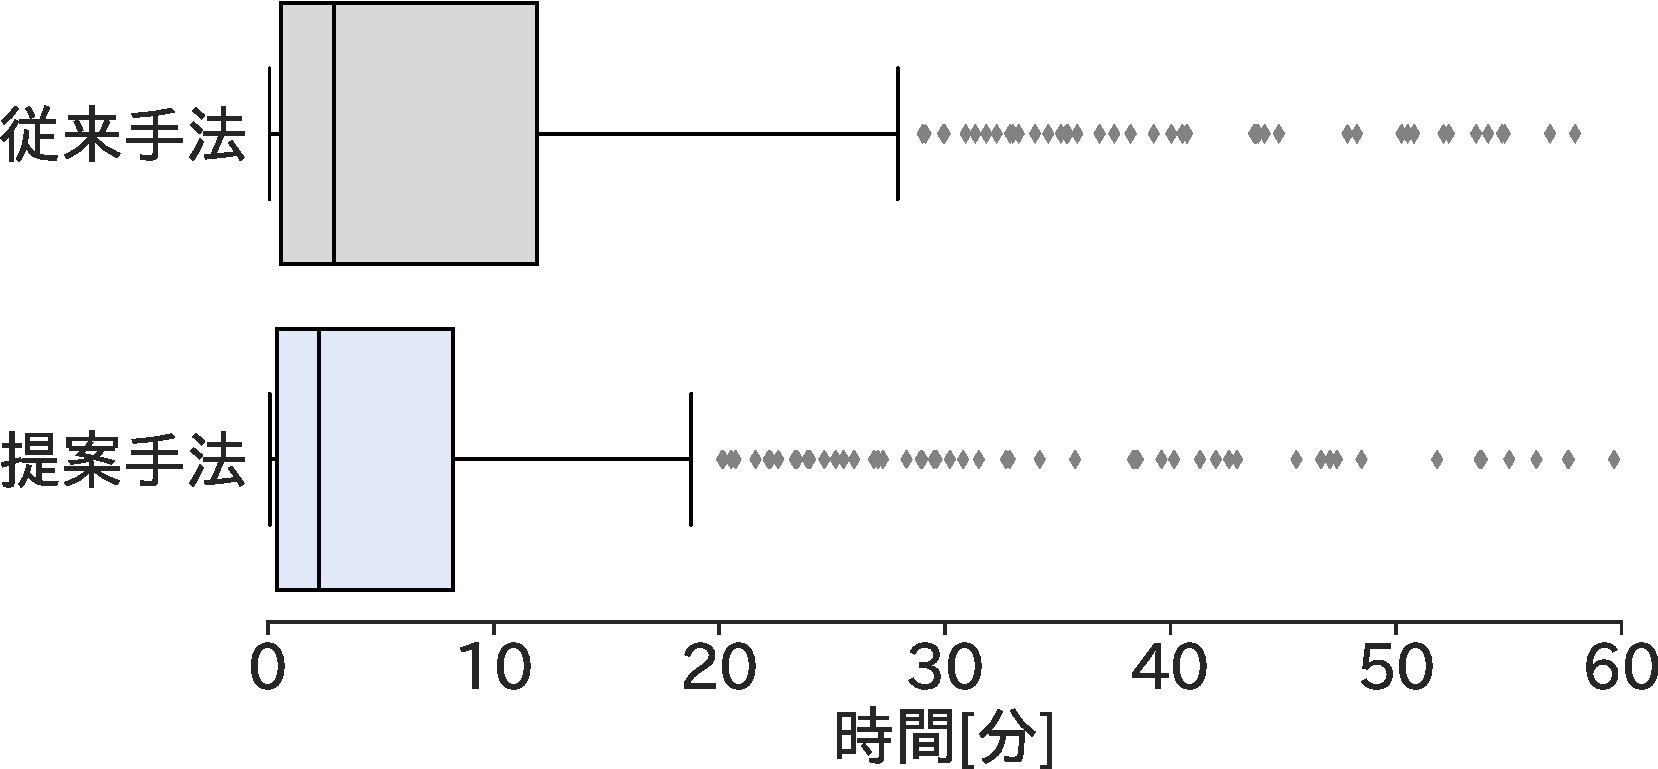
\includegraphics[width=.5\linewidth]{fig-boxp.pdf}
  \caption{生成時間の比較}
  \label{fig:time_all}
\end{figure}


\bibliographystyle{sieicej}
\bibliography{references}

\end{document}
